\documentclass[a4paper,12pt,oneside]{book}%


\parskip 10 pt           % sets spacing between paragraphs

\usepackage{graphicx}
\usepackage{indentfirst}
\usepackage[romanian]{babel}
\usepackage{longtable}
\usepackage{verbatim}
\usepackage{listings}
\usepackage{indentfirst}
\usepackage{float}
\usepackage{amsmath}
\usepackage{amsfonts}
\usepackage{amssymb}
\usepackage{color}
\usepackage[nottoc]{tocbibind}
\usepackage[T1]{fontenc}
\usepackage{fancyhdr}
\usepackage{epstopdf}
\usepackage[obeyspaces,hyphens]{url}
\usepackage[utf8x]{inputenc}
\usepackage{caption}
\usepackage{subcaption}
\usepackage{lmodern}
\usepackage{dsfont}
%\usepackage{fullpage}
\usepackage{algorithm}% http://ctan.org/pkg/algorithm
\usepackage{algpseudocode}% http://ctan.org/pkg/algorithmicx
\usepackage{tabularx}
\usepackage{placeins}
\usepackage{float}
\floatstyle{boxed}
\restylefloat{figure}

\usepackage{natbib}
\usepackage{bibentry}


\usepackage{verbatim}
\usepackage{moreverb}
\let\verbatiminput=\verbatimtabinput
\def\verbatimtabsize{4\relax} 

\usepackage{mdframed}

\usepackage{natbib}

\usepackage{listings}
\usepackage{color}

\definecolor{mygreen}{rgb}{0,0.6,0}
\definecolor{mygray}{rgb}{0.5,0.5,0.5}
\definecolor{mymauve}{rgb}{0.58,0,0.82}


\lstset{
	backgroundcolor=\color{white},
	basicstyle=\footnotesize,
	commentstyle=\color{mygreen},
	frame=single,
	numbers=left,
	numbersep=5pt,
	numberstyle=\tiny\color{mygray},
	rulecolor=\color{black},
	tabsize=2,
	stringstyle=\color{mymauve},
	breaklines=true
}

\widowpenalty=700
\clubpenalty=700

%\RequirePackage[l2tabu, orthodox]{nag}

\setlength{\headheight}{15.35403pt}

\renewcommand{\chaptermark}[1]{%
\markboth{#1}{}}
\fancyhead{}
\fancyhead[L]{\rightmark}

\usepackage{enumitem}
\setlist{topsep=0pt}


\addto\captionsromanian{%
  \renewcommand{\tablename}%
    {Tabelul}%
}

%\setlength{\parskip}{0pt}
%\setlength{\parsep}{0pt}
%\setlength{\headsep}{0pt}
%\setlength{\topskip}{0pt}
%\setlength{\topmargin}{0pt}
%\setlength{\topsep}{0pt}
%\setlength{\partopsep}{0pt}

\usepackage[compact]{titlesec}
%\titlespacing{\chapter}{0pt}{*4}{*4}
%\titlespacing{\section}{0pt}{*2}{*2}
%\titlespacing{\subsection}{0pt}{*1}{*1}
%\titlespacing{\subsubsection}{0pt}{*1}{*1}

%\addto\extrasromanian{%  
%  \def\tableautorefname{Tabela}%
%  \def\figureautorefname{Figura}%  
%  \def\equationautorefname{Ecuația}%  
%  \def\tableautorefname{tabela}%
%  \def\figureautorefname{figura}%  
%  \def\equationautorefname{ecuația}%  
%}

\usepackage[unicode,colorlinks=false,pdfauthor={Draghia Alin-Madalin},pdfsubject={Tehnici de Machine Learning in procesarea si recunoasterea imaginilor},pdfcreator=Miktex,pdfproducer=Miktex,pdfkeywords={ML, Machine Learning, Object Detection, SVM, Sliding Window, Feature Extraction, Object Recognition},pdfcenterwindow=true,pdfstartview=FitH]{hyperref}
\usepackage[all]{hypcap}

\newcommand{\superscript}[1]{\ensuremath{^{\textrm{#1}}}}
\newcommand{\subscript}[1]{\ensuremath{_{\textrm{#1}}}}



\title{Tehnici de Machine Learning in procesarea si recunoasterea imaginilor}
\author{Draghia Alin-Madalin}

\usepackage{pdfpages}

\begin{document}

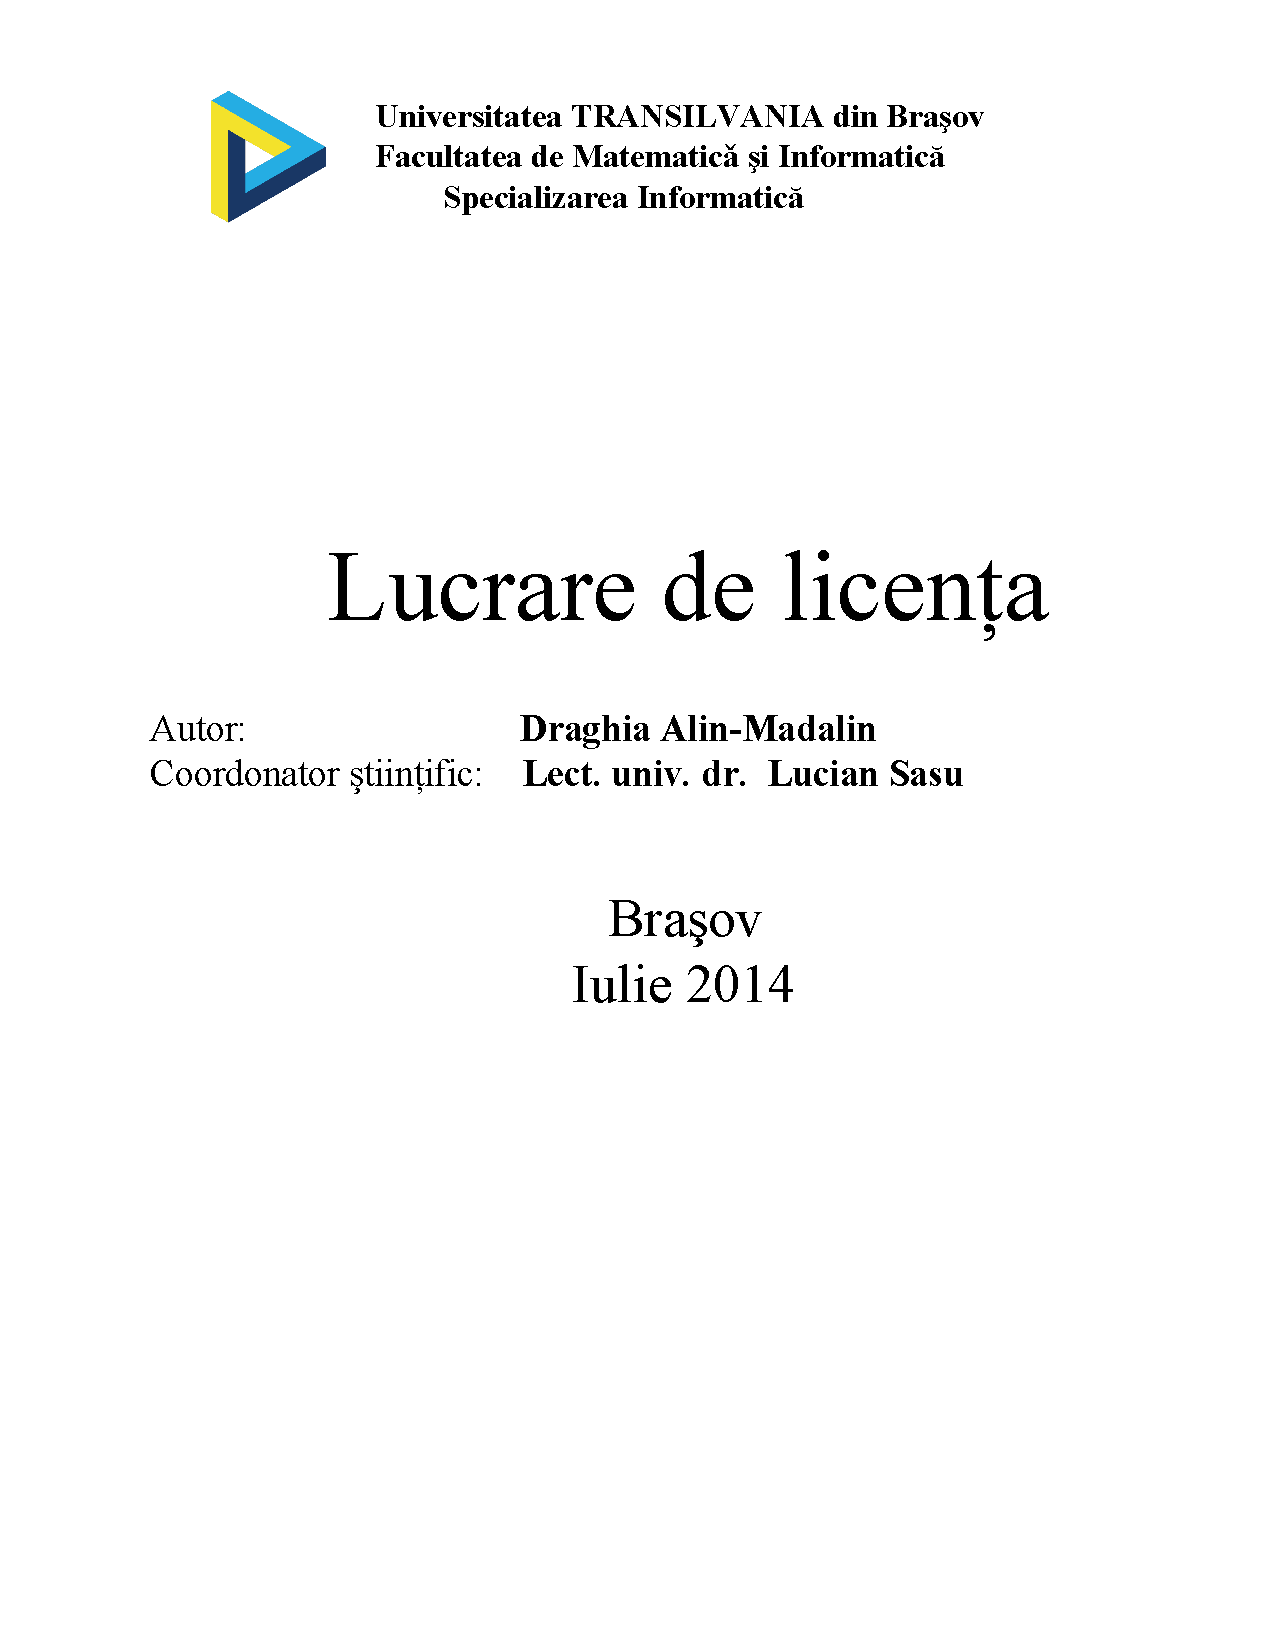
\includepdf[pages={1}]{coperta.pdf}

\fancyfoot{}
\pagenumbering{alph}
\setcounter{page}{1}
\pagestyle{empty}

\begin{titlepage}

\begin{center}

\Large Universitatea Transilvania din Brașov

\Large Facultatea de Matematică și Informatică

\large Specializarea Informatică

\vfill
\Large Proiect de Licență\\[0.3cm]
 
{ \Huge \bfseries Tehnici de Machine Learning în procesarea și recunoașterea imaginilor}\\[2cm]
 
\begin{minipage}{0.4\textwidth}
\begin{flushleft} \large
\emph{Autor:}\\
Draghia Alin-Mădălin
\end{flushleft}
\end{minipage}
\begin{minipage}{0.5\textwidth}
\begin{flushright} \large
\emph{Profesor coordonator:} \\
Lect. Dr. Sasu Lucian Mircea
\end{flushright}
\end{minipage}
 
\vfill

{\Large Brașov}

{\large Iulie 2014}
 
\end{center}
 
\end{titlepage}
\pagestyle{fancy}

\pagenumbering{roman}
\setcounter{page}{1}
\newpage
\pagestyle{empty}
{
\renewcommand{\headrulewidth}{0pt}
\fancypagestyle{plain}
{
    \fancyhead{}
    \fancyfoot{}
}	% clear header and footer of plain page because of ToC\pagestyle{empty}
\tableofcontents
}
\newpage
\cleardoublepage
\pagestyle{fancy}
\fancyfoot[C]{\thepage}
\pagenumbering{arabic}
\setcounter{page}{1}



\chapter{Introducere}

%Aceasta lucrare își propune sa prezinte, din punct de vedere atât teoretic cat și practic în ce consta dezvoltarea unui algoritm de recunoaștere a obiectelor în imagini, folosind tehnici de procesare a imaginilor și învățare automata.

Prin intermediul acestei lucrări doresc să prezint, din punct de vedere teoretic, pașii necesari în dezvoltarea unui sistem de recunoaștere a obiectelor în imagini, folosind tehnici de procesare a imaginilor și învățare automată.

Totodată, această lucrare vine însoțită de implementarea unei biblioteci software pentru dezvoltarea de algoritmi și aplicații de recunoaștere a obiectelor.
În plus, pe baza acestei biblioteci, am implementat unul dintre algoritmii de recunoaștere consacrați.



\section{Motivație}

Recunoașterea obiectelor este una dintre principalele aplicații ale viziunii artificiale și procesarea de imagini. 

Oamenii pot recunoaște o mulțime de obiecte într-o imagine fără sa depună prea mult efort, chiar dacă în aceste imagini obiectele prezintă variații de perspectiva, de dimensiune, sunt translatate, rotite sau chiar obstrucționate. 
Cu toate că de-a lungul timpului au fost studiați și dezvoltați multi algoritmi, sistemele de recunoaștere automată a obiectelor sunt încă departe de performanta unei ființe umane, chiar de cea a unui copil de numai doi ani.
Așadar, încă există loc pentru cercetarea și dezvoltarea algoritmilor în acest domeniu.

%În ciuda performantei relativ scăzute a acestor algoritmi, odată cu dezvoltarea sistemelor hardware, fapt ce a permis aplicarea unor algoritmi mult mai complicați sau au putut fi aplicați pe niște probleme de dimensiune mai mare, cererea de aplicații a crescut. 

Odată cu dezvoltarea sistemelor hardware, fapt ce a permis aplicarea unor algoritmi mult mai complicați sau a făcut posibilă aplicarea celor deja existenți pe niște probleme de dimensiune mult mai mare, cererea de aplicații a crescut.
Câteva dintre cele mai de succes aplicații sunt: 
\begin{itemize}
	\item Sistemul de frânare automată la detecția pietonilor instalat pe mașinile Volvo.\cite{volvo}
	\begin{figure}[H]
		\centering
			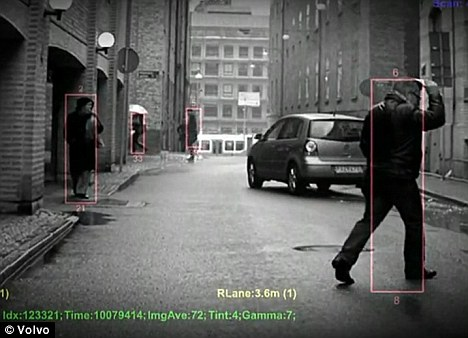
\includegraphics[width=0.8\textwidth]{imagini/volvo_pedestrian_detection.jpg}
		\caption{Volvo: sistemul de detecție a pietonilor\cite{VolvoArticle}}.
		\label{fig:volvo_pedestrian_detection}
	\end{figure}
	
	\item Focalizarea automată a camerelor foto pe fețe		
	\begin{figure}[H]
		\centering
			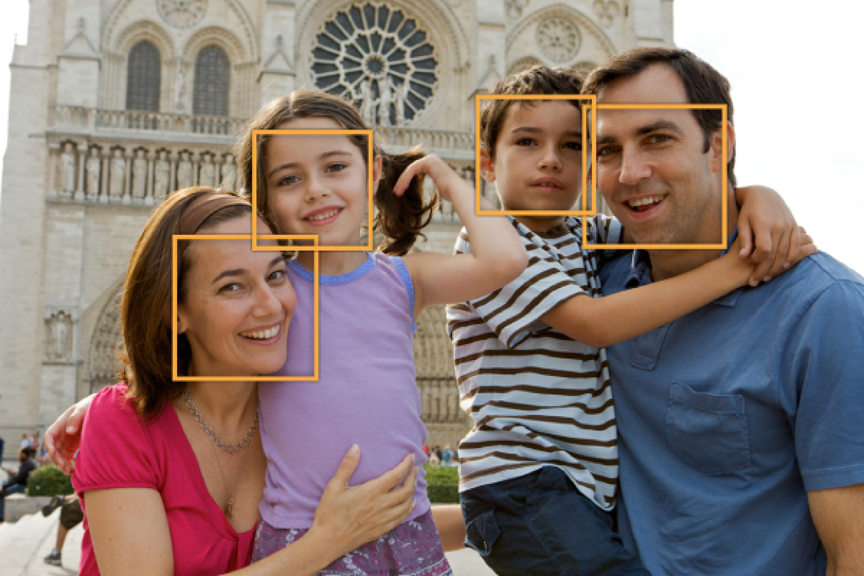
\includegraphics[width=0.8\textwidth]{imagini/face_detection_2x.png}
		\caption{Cameră foto: focus automat\cite{CanonFaceRecognition}}
		\label{fig:face_detection_2x}
	\end{figure}
	


	\item Analizarea traficului rutier	
	\begin{figure}[H]
		\centering
			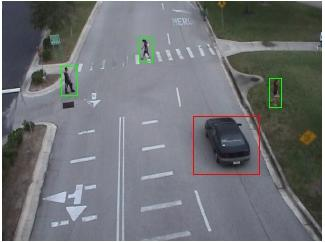
\includegraphics[width=0.9\textwidth]{imagini/traffic_analisys.jpg}
		\caption{Analizarea traficului rutier\protect\footnotemark}
		\label{fig:traffic_analisys}
	\end{figure}

\end{itemize}
	\footnotetext{\url{http://youtu.be/PXSiUojhNFg}}

Înțelegerea și dezvoltarea unui sistem de recunoaștere automată a obiectelor poate fi foarte dificilă, mai ales pentru cei care sunt la început de drum în studierea acestui domeniu. 
Documentația de specialitate, de cele mai multe ori, este scrisă privind problema de la un nivel foarte înalt și nu sunt tratate detaliile algoritmilor. 
În același timp, în foarte multe lucrări se fac referiri la lucrări anterioare, unele chiar cu zeci de ani distantă intre ele, acestea fiind uneori foarte greu de găsit.
Parcurgerea unui astfel de document presupune cunoștințe extensive de matematică, statistică, învățare automată, procesarea imaginilor și chiar cunoștințe din domeniul biologic sau medical. 
Toate acestea fac ca nivelul de la care se intră acest domeniu sa fie unul foarte înalt, ceea ce poate fi descurajant pentru un începător.

Exista câteva biblioteci software bune, "open-source", cu care se pot dezvolta aplicații: 
opencv\footnote{\url{http://opencv.org/}}, 
dlib\footnote{\url{http://dlib.net/}}, 
libccv\footnote{\url{http://libccv.org/}}.
Avantajele lor sunt:
\begin{itemize}
	\item Există algoritmi de recunoaștere a obiectelor gata implementați.
	\item Se poate trece direct la dezvoltarea de aplicații
\end{itemize}
Totuși sunt și dezavantaje:
\begin{itemize}
	\item Componentele care stau la baza acestor implementări nu sunt expuse, reutilizarea lor fiind imposibilă.
	\item Codul sursă este optimizat cu instrucțiuni de asamblare sau pentru procesorul grafic, fiind dificil de înțeles.
\end{itemize}
Aceste dezavantaje fac ca aceste biblioteci sa nu fie utile celor care doresc sa dezvolte sau să studieze astfel de algoritmi.

La finalul lucrării s-a obținut o platformă de dezvoltare a algoritmilor pentru recunoașterea obiectelor, pe care să o pot folosi în activitatea mea din domeniu și care să servească drept punct de plecare pentru cei care doresc să se inițieze în domeniu.

Avantajele acestei platforme ar fi:
\begin{itemize}
	\item Fiecare componentă a unui algoritm de recunoaștere este implementat într-o clasă separată
	\item Algoritmii pot fi implementați atât în C++ cât și în Python
	\item Reutilizare sporită a componentelor
	\item Pot fi ușor adaptați algoritmi din alte biblioteci pentru utilizare în cadrul platformei
\end{itemize}

C++ și Python sunt două limbaje de programare foarte diferite, dar tocmai aceste diferențe fac ca cele două să se îmbine aproape perfect, formând un mediu de lucru prielnic studierii și dezvoltării de algoritmi.

%Viziunea artificiala reprezinta procesul invers al celui de formare a imagini și se ocupa cu recuperarea de informații din imagini cu ajutorul metodelor matematice, geometrice, statistice și a teoriei învățării automate\footnote{Machine learning}.

%Recunoașterea automata a obiectelor se refera la capacitatea unui sistem software de localizare și identificare a obiectelor într-o imagine sau o secventa video.

%Din punct de vedere practic, aceasta lucrare își propune dezvoltarea unei biblioteci software și aplicații demonstrative, cu ajutorul cărora sa se poată dezvolta aplicații de recunoașterea obiectelor în imagini.

%Din punct de vedere teoretic sunt descrise componentele și structura unui astfel algoritm, precum și cel folosit pentru al antrena.



%Viziunea artificiala și învățarea automata sunt doua domenii aflate în plina dezvoltare și sunt de mare interes atât în cadrul academic ca și în industria software.

%Dezvoltarea rapida a sistemelor de calcul a permis utilizarea acestor algoritmi în tot mai multe aplicații. Câteva dintre aplicațiile recunoașterii de obiecte sunt:
%\begin{itemize}
%	\item Industriale: recunoașterea și verificarea cip-urilor pe o placa electronica, numărarea de obiecte pe o banda rulanta
%	\item Securitate: recunoașterea unui intrus folosind o camera de supraveghere
%	\item Medicale: recunoașterea diferitelor tumori într-o imagine de tomografie
%	\item Fotografie: focalizare automata pe fete
%	\item Internet: căutare google după imagini, marcarea automata a fetelor într-o poza de pe facebook
%\end{itemize}

%Interesul 

%Pana acum am folosit și am studiat o mulțime de algoritmi de recunoaștere a obiectelor, dar pentru a aprofunda înțelegerea acestor algoritmi cel mai bine este sa fie scris măcar unul de la un capăt la altul.

%Cei mai multi algoritmi de recunoaștere a obiectelor au o structura comuna formata din următoarele componente: scanarea imaginii, extragerea de trasaturi, classificare si procesarea rezultatelor.

%Multi algoritmi sunt scrisi intr-un mod foarte rigid si componentele lor nu pot fi refolosite. Sunt optimizati pana la punctul in care codul sursa nu mai poate fi inteles cu usurinta.

%In cadrul companiei la care lucrez, Dynamic Ventures, am folosi

%Desi, am folosit si m-am documentat 

%Am ales sa dezvolt o astfel de librarie, chiar daca exista si altele, din doua motive.





%Aceasta problema nu poate fi nici pe departe considerata rezolvata, de-a lungul timpului un număr mare de algoritmi au fost propuși.

%Mult timp recunoașterea automata a obiectelor în imagini a fost considera impracticabila datorita complexității de timp și spațiu a acestor algoritmi.






\section{Enunțul problemei}
Se scrie o bibliotecă software cu ajutorul căreia să se dezvolte algoritmi și aplicații de recunoaștere a obiectelor.

Această bibliotecă va fi scrisă într-un mod hibrid, cu componente implementate atât în C++ cât și în Python.
Această combinație de limbaje va permite implementarea rapidă a algoritmilor în Python, iar la nevoie aceștia pot fi implementați parțial în C++.

Toate componentele bibliotecii vor suporta serializare pentru a putea fi salvate pe disc, baze de date sau trimise prin rețea în cazul unor programe distribuite.
De asemenea se serializează rezultatul unor sesiuni lungi de antrenare.

Algoritmul va învăța sa recunoască obiecte folosindu-se de un set de imagini cu exemple pozitive adnotate și exemple negative, imagini care nu conțin obiectul pe care dorim sa-l învățam.
Algoritmul poate fi personalizat prin alegerea de implementări diferite ale componentelor de către utilizator.

Ca exemplificare, se scrie o aplicație care antrenează un algoritm de recunoaștere și salvează modelul învățat pe disc și o altă aplicație care încarcă modelul și îl aplică pe o imagine data.



\section{Structura Lucrării}


Capitolele care urmează vor trata algoritmii de recunoaștere a obiectelor din punct de vedere teoretic și se va prezenta implementarea unei platforme de dezvoltare a acestora.

În capitolul 2 sunt prezentate în detaliu structura algoritmilor de recunoaștere și o tehnică eficienta de antrenare.

În capitolul 3 sunt prezentate tehnologiile folosite.

În capitolul 4 sunt prezentate în detaliu structura cadrului de lucru, implementarea unui algoritm de recunoaștere și modalități de extindere a bibliotecii.

În capitolul 5 sunt prezentate concluzii despre lucrare, precum și posibilități de dezvoltare.

\pagebreak
\chapter{Recunoașterea obiectelor}


%Recunoașterea obiectelor este o aplicate fundamentala a procesării de imagini și viziunea artificiala.
%De câteva decenii a fost, și încă este un domeniu de cercetare extensiva.
%Termenul "recunoașterea obiectelor" este folosit pentru a descrie multe aplicații și algoritmi.
%Sensul comun, de cele mai multe ori, este: date find cunoștințe despre înfățișarea unor obiecte, una sau mai multe imagini sunt analizate pentru a se stabili dacă exista obiectele în imagine și locația lor.
%Cu toate acestea, fiecare aplicație are cerințe și constrângeri specifice.
%Acest fapt a condus la o mare diversitate de algoritmi.
%De aceea este important ca sa avem la îndemâna biblioteci software, care sa faciliteze dezvoltarea rapida a algoritmilor de recunoaștere a obiectelor.

%Un caz special de recunoaștere a obiectelor apare foarte des, baza de date a modelelor ce trebuiesc recunoscute conține o singura clasa de obiecte, în acest caz sarcina de a detecta prezenta obiectului în imagine este simplificata.

Problema recunoașterii de obiecte se poate exprima în felul următor: Având un o baza de date cu unul sau mai multe modele de obiecte, sa se determine dacă exista obiectul în imagine și dacă exista sa se localizeze.

Unele dintre cele mai relevante lucrări din domeniu sunt: 
\begin{itemize}
	\item "Robust Real-time Object Detection" \cite{Viola01robustreal-time}
	\item "Histograms of Oriented Gradients for Human Detection" \cite{Dalal05histogramsof}
	\item "Object Detection with Discriminatively Trained Part Based Models" \cite{Felzenszwalb_objectdetection}
\end{itemize}

Dacă studiem mai atent algoritmii descriși în aceste lucrări se observa ca toate au o structura comuna și urmăresc o succesiune de operațiuni similare.
Aceste operațiuni sunt următoarele: parcurgerea imaginii în scara și spațiu, extragerea de trăsături, clasificare și post-procesarea rezultatelor.

În continuare se va discuta mai detaliat despre fiecare componenta, iar la sfârșit despre algoritmul de recunoaștere.

\pagebreak
\section{Parcurgerea imaginii în scara și spațiu}

%Obiectele trebuie recunoscute la orice poziție și scara într-o imagine.
Obiectele care trebuiesc recunoscute pot prezenta deviații de la modelul din baza de date, aceste deviații pot fi de natura geometrica: translație, rotație, scalare și perspectiva.

O soluție pentru aceasta problema ar fi sa se construiască un model care sa prezinte toate instanțierile obiectului.
O dificultate cu aceasta abordare ar fi ca nu se pot știi dinainte toate transformările obiectului, chiar dacă s-ar știi, se poate deduce ca un astfel de model ar putea fi mult prea mare ca sa poată fi aplicat practic.

O alta abordare a fi sa se folosească o reprezentare a imaginii invarianta la aceste transformări.
Din literatura se știe ca o imagine reprezentata în spațiul Fourier este invarianta la translație și o imagine reprezentata în spațiul Log-Polar este invarianta la scalare și rotație.
Exista chiar și o combinație intre aceste doua reprezentări numita Fourier-Mellin care este invarianta la toate cele trei transformări.
Totuși s-a observat ca utilizarea acestei reprezentări are aplicații limitate, ea find folosita mai mult la alinierea imaginilor.

O alta soluție, poate un pic mai naiva, dar în același timp foarte puternica este folosirea unei combinații de piramida de imagini și un algoritm de tip fereastră glisantă\footnote{eng. sliding window}, acestea find aplicate pe imagine, nu pe modelul din baza de date.

Folosirea piramidei de imagini și fereastra glisanta ne permite ca in restul algoritmului de recunoaștere sa tratam problema ca și cum nu ar exista translații sau scalari, astfel simplificând mult algoritmii aplicați.

O piramida de imagini este o reprezentare multi-scara.
Piramida de imagini se formează, pornind de la o imagine sursa, prin scalari succesive.
Aceste scalari se fac cu un factor și se opresc atunci când se ajunge la o dimensiune minima.
Dacă factorul de scalare este ${\alpha > 1}$ atunci avem funcția care calculează dimensiunea unui nivel este  
$${ f(D,L) = D * \frac{1}{\alpha^L} }$$, unde ${D}$ este dimensiune imaginii sursa și ${L}$ este nivelul piramidei pentru care dorim sa aflam dimensiune.

Se poate vizualiza piramida de imagini în figurile următoare:

\begin{figure}[H]
	\centering
		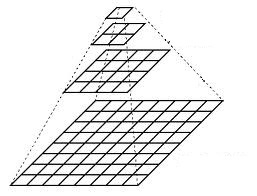
\includegraphics[width=0.90\textwidth]{imagini/Pyramids_Tutorial_Pyramid_Theory.png}
	\caption{Piramida de imagini}
	\label{fig:Pyramids_Tutorial_Pyramid_Theory}
\end{figure}

\begin{figure}[H]
	\centering
		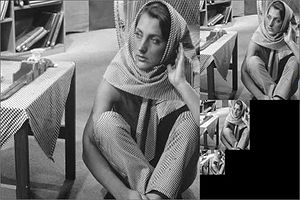
\includegraphics[width=0.90\textwidth]{imagini/300px-Example_pyramid.jpg}
	\caption{Exemplu piramida de imagini}
	\label{fig:300px-Example_pyramid}
\end{figure}


Prezentarea formarii piramidei de imagini în pseudo-cod:
\begin{mdframed}
\begin{verbatim}
sursa = citeste_imagine()
alpha = 6/5
dim_min = (100,100)
piramida = [sursa, ]
L=1
cicleaza
  D = sursa.D * 1/(alpha^L)
  daca D < dim_min
    atunci paraseste ciclul
  sfarsit daca
  nivel = scaleaza(sursa, D)
  piramida = insereaza(piramida, nivel)
  L = L + 1
sfarsit cicleaza
\end{verbatim}
\end{mdframed}

Se poate observa ca totuși acest model nu poate reprezenta toate scările posibile, find un model discret, aceasta problema poate fi ameliorata prin alegerea unui ${\alpha}$ potrivi și permițând modelului din baza de date sa reprezinte și el mici variații de scara.

O alta observație ar fi, cu cat ${\alpha}$ este mai mic, cu atât șansele sa nimerim scara corecta cresc, dar în același timp creste și consumul de memorie și durata de execuție a algoritmului. Consumul de memorie poate fi evitat dacă algoritmul se executa într-un mod recursiv, astfel eliminând menținerea explicita a unei liste de imagini în memorie.

Algoritmul fereastra glisanta se folosește pentru a obține invarianta la translație a modelului.
Aici fereastra se refera la o secțiune rectangulara a imaginii.
Fereastra va avea aceiași dimensiune ca și modelul din baza de date.
Fereastra glisanta are ca parametri ${\Delta_x, \Delta_y \geq 1}$, însemnând pasul pe axa x, respectiv pasul pe axa y.

Pseudo-cod fereastra glisanta:
\begin{mdframed}
\begin{verbatim}
dx = 8
dy = 8
I = citeste_imagine()
M = citeste_model()
pentru x de la 0 la dimx(I) - dimx(I)
  pentru y de la 0 la dimy(I) - dimy(M)
    fereastra = sectiune(I, x, y, dimx(M), dimy(M))
    proceseaza(fereastra)
  sfarsit pentru
sfarsit pentru
\end{verbatim}
\end{mdframed}

Se poate vizualiza algoritmul fereastra glisanta în figura următoare:
\begin{figure}[H]
	\centering
		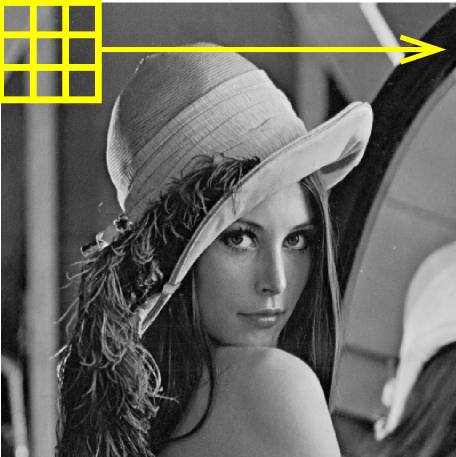
\includegraphics[width=0.70\textwidth]{imagini/AGhannoum-SlidingWindow.png}
	\caption{Fereastra glisanta}
	\label{fig:AGhannoum-SlidingWindow}
\end{figure}


Se observa ca și aici, ca și în cazul piramidei de imagini, cu cat x și y sunt mai mici cu atât creste și numărul de ferestre evaluate, ceea ce duce la un timp de execuție mai ridicat.

Complexitatea algoritmului piramida combinat cu fereastra glisanta este 
$${O((dim_x-\Delta_x)*(dim_y-\Delta_y)*n_{piramida})}$$

\pagebreak
\section{Extragerea de trăsături}

Extragerea de trăsături se ocupa cu, în cazul nostru, calcularea unei reprezentări a imaginii potrivite pentru recunoaștere.

O imagine este reprezentata ca o matrice de intensități.
Aceasta reprezentare este foarte sensibila la condițiile de iluminare, conține informații irelevante și redundante.
Se poate observa efectul iluminării în figura \ref{fig:efectul_iluminarii}.

\begin{figure}[H]
	\centering
		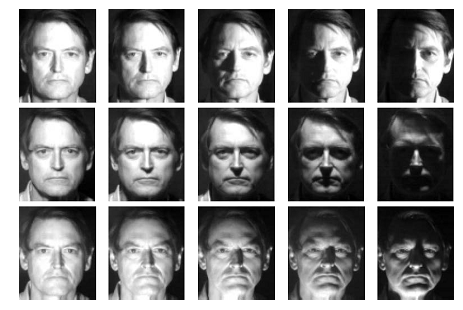
\includegraphics[width=0.90\textwidth]{imagini/efectul_iluminarii.png}
	\caption{Efectul iluminarii}
	\label{fig:efectul_iluminarii}
\end{figure}

Exista modalități de a remedia efectul iluminării, cum ar fi egalizarea histogramei(fig. \ref{fig:egalizarea_histogrameis}).
O alta modalitate ar fi sa se folosească o reprezentare pe baza de gradienți care sunt invarianți la iluminare.

\begin{figure}[H]
	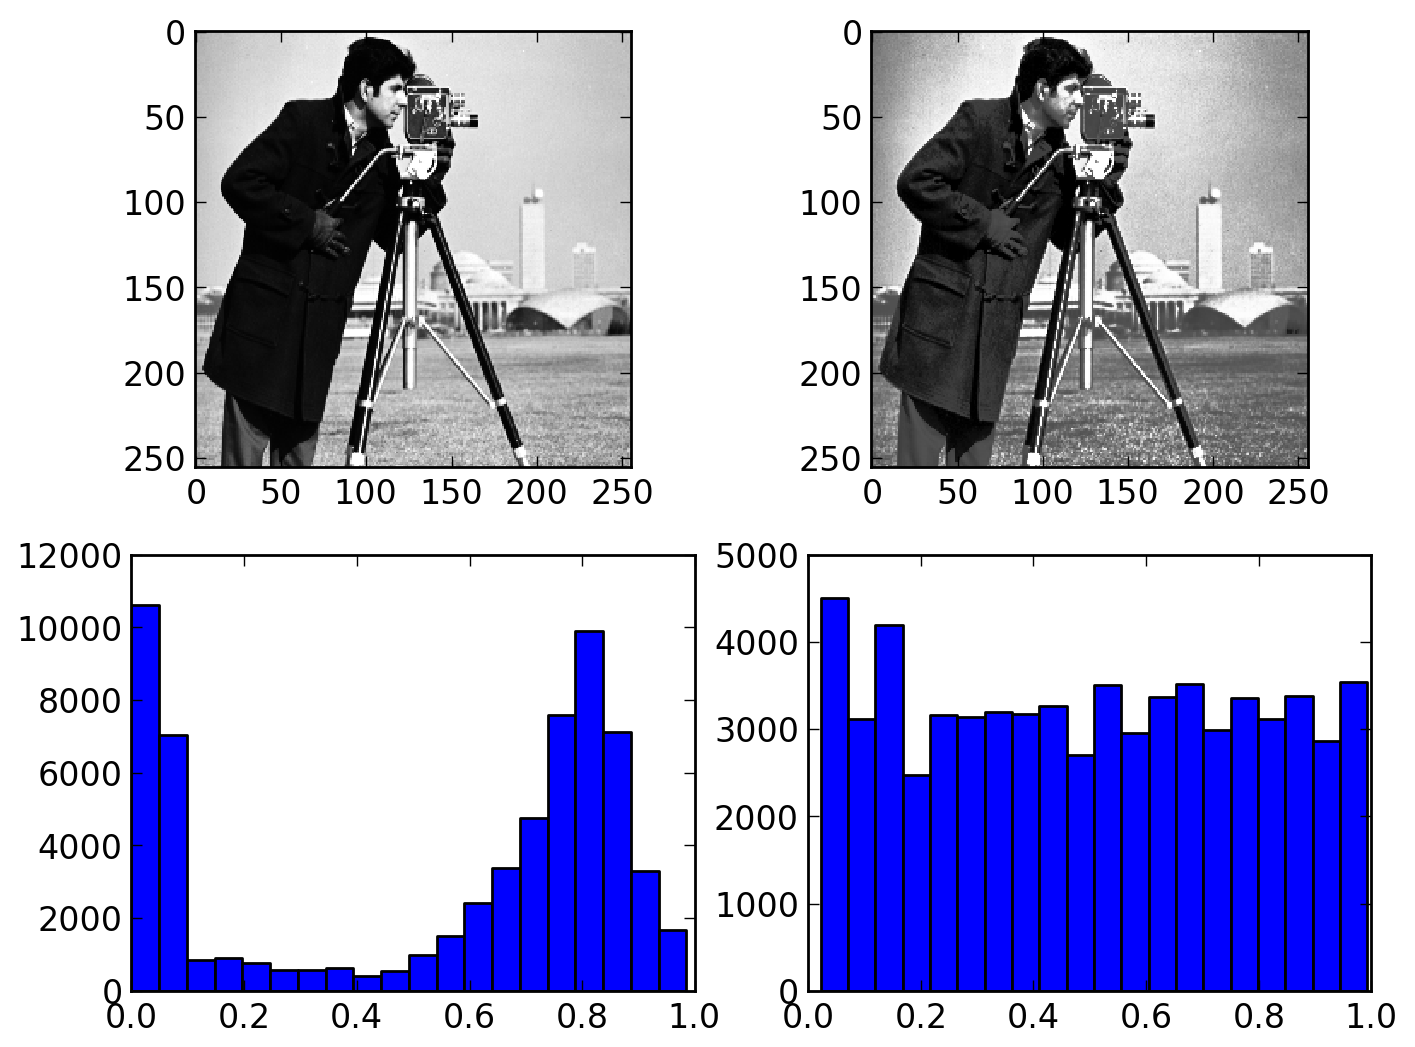
\includegraphics[width=0.90\textwidth]{imagini/HistogramEqualization-1.png}
	\caption{Egalizarea Histogramei}
	\label{fig:egalizarea_histogrameis}
\end{figure}


Efectul informațiilor irelevante și redundante poate fi ameliorat folosind tehnici de reducerea de dimensionalitate, cum ar fi analiza componentelor principale\footnote{eng. PCA, principal component analisys}(fig. \ref{fig:fig_pca_principal_component_analysis} sau transformata cosinus discreta(fig. \ref{fig:take_DCT}).

\begin{figure}[H]
	\centering
		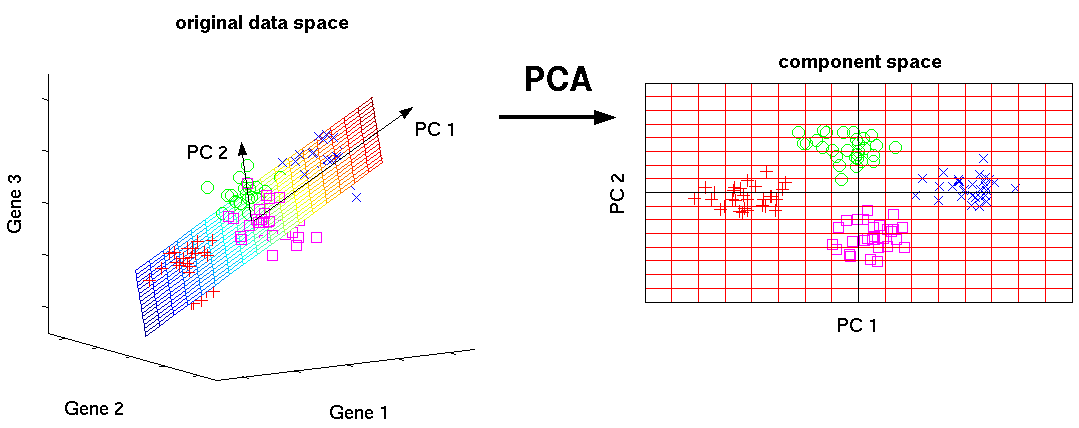
\includegraphics[width=0.90\textwidth]{imagini/fig_pca_principal_component_analysis.png}
	\caption{Analiza componentelor principale}
	\label{fig:fig_pca_principal_component_analysis}
\end{figure}

\begin{figure}[H]
	\centering
		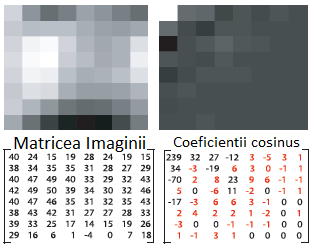
\includegraphics[width=0.90\textwidth]{imagini/take_DCT.png}
	\caption{Transformata cosinus}
	\label{fig:take_DCT}
\end{figure}



Totuși nici una dintre reprezentările menționate mai sus nu tratează problema discriminării, adică dacă doua imagini conțin același obiect atunci și reprezentările lor trebuie sa fie apropiate, iar dacă sunt imagini ale unor obiecte diferite atunci reprezentările lor sa fie distanțate.

Aici intervine ceea ce se numește ingineria trăsăturilor\footnote{eng. Feature Engineering} care, folosind cunoștințe din fizica, biologie sau chiar neurologie construiește reprezentări mult mai favorabile recunoașterii.
Câteva dinte cele mai cunoscute trăsături sunt Haar\cite{Viola01robustreal-time}, Sift\cite{Lowe99objectrecognition} și Hog\cite{Dalal05histogramsof}.

Valoare unei trăsături Haar este diferența dintre suma pixelilor din dreptunghiul negru și suma pixelilor din dreptunghiul alb, normalizata la aria celor doua.
\begin{figure}[H]
	\centering
		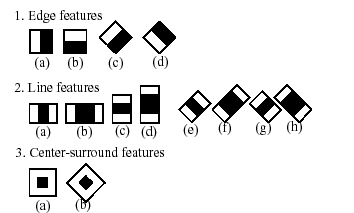
\includegraphics[width=0.90\textwidth]{imagini/haarfeatures.png}
	\caption{Trasaturi Haar}
	\label{fig:haarfeatures}
\end{figure}

Hog, sau histograma orientărilor de gradienți, se calculează divizând imaginea in zone mai mici, numite celule, apoi se calculează histograma de orientări a gradienților din aceste zone. 
Concatenarea acestor histograme reprezentând trăsătura hog.
\begin{figure}[H]
	\centering
		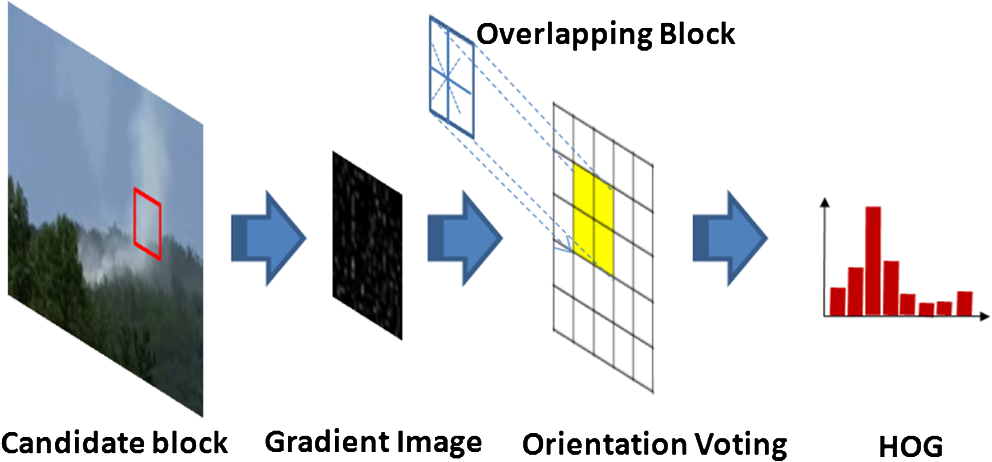
\includegraphics[width=0.90\textwidth]{imagini/OE_51_1_017208_f004.png}
	\caption{Trasaturi hog}
	\label{fig:OE_51_1_017208_f004}
\end{figure}

Descriptorul Sift este similar cu Hog, acesta find în plus și invariant la rotație.
\begin{figure}[H]
	\centering
		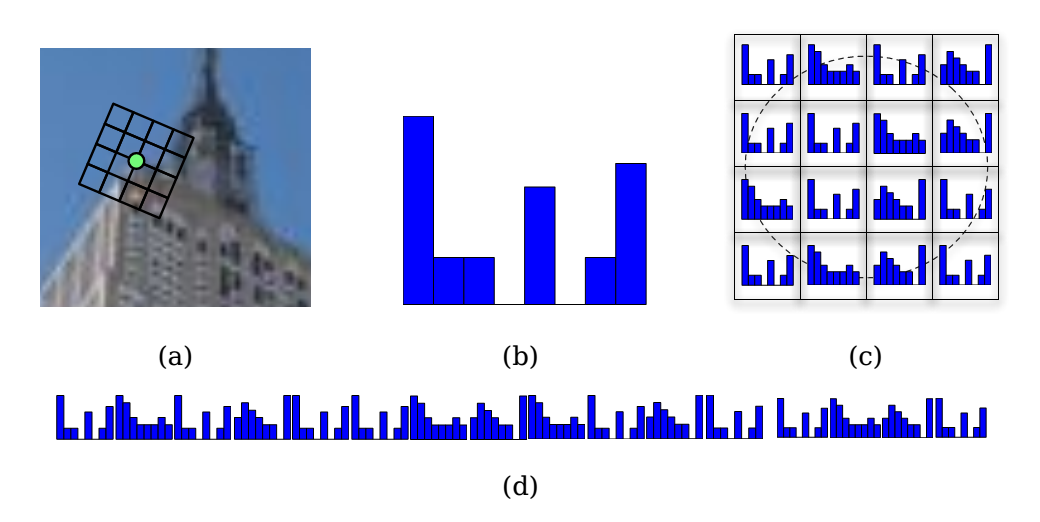
\includegraphics[width=0.90\textwidth]{imagini/sift.png}
	\caption{Descriptorul Sift}
	\label{fig:sift}
\end{figure}

Recent a apărut o noua abordare, în ceea ce privește extragerea de trăsături, aceasta folosește reprezentarea cruda a imaginii, adică matricea de intensități a pixelilor și se bazează pe algoritmul de clasificare sa extragă trăsături mai puternice, un exemplu ar fi rețeaua neurala convolutionala.\cite{lecun-98}

\pagebreak
\section{Clasificare}

Din perspectiva recunoașterii obiectelor, clasificarea se va realiza cu ajutorul unei funcții care evaluează un vector de trăsături și decide dacă este sau nu obiectul pe care încercam sa îl recunoaștem. 
Acest tip de clasificare se numește clasificare binara, findcă răspunsul nu poate lua decât doua valori.

Aceasta funcție de decizie poate fi, în cazurile cele mai simple, o funcție de prag peste o distanta euclidiana sau chiar o rețea neuronala cu sute de neuroni.

În cazul nostru aceasta funcție este rezultatul unui algoritm de învățare automata.\footnote{Machine Learning}
Învățarea automata, o ramura a inteligentei artificiale, este preocupata cu construcția și studiul sistemelor care pot învață din date.
Algoritmii de învățare automata sunt împărțiți în multe categorii, însa noi ne vom axa doar pe cei de învățare supervizata.
Se numesc algoritmi de învățare supervizata, acei algoritmi care folosesc la antrenament seturi de perechi de date ${(x,y)}$ unde ${x}$ reprezinta trăsăturile sau atributele unui exemplar, iar ${y}$ reprezinta răspunsul dorit. 
După ce a avut loc învățarea, algoritmul va fi capabil sa producă un răspuns și în cazul unor exemplare pe care nu le-a mai întâlnit, de aceea în literatura de specialitate clasificatori se mai numesc și predictori.

Scopul învățării automate, dacă privim problema din punct de vedere geometric, este acela de a găsi o un plan care sa separe cele doua clase intre ele.

\begin{figure}[h]
	\centering
		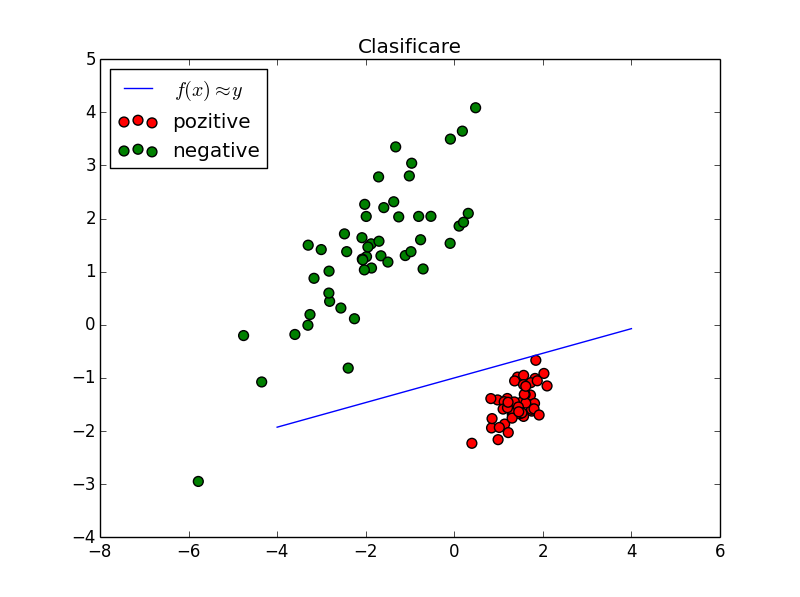
\includegraphics[width=0.90\textwidth]{imagini/fig_clasificare.png}
	\caption{Clasificare}
	\label{fig:fig_clasificare}
\end{figure}

Cel mai des întâlniți algoritmi de învățare în viziunea artificiala sunt: automatul cu vectori de suport\footnote{eng. Support Vector Machines}, rețeaua neuronala.

\pagebreak
\section{Post-procesarea rezultatelor}

O situație foarte des întâlnita în cazul algoritmilor de recunoaștere a imaginilor este ca același obiect este detectat de mai multe ori.
Aceste detecții sunt suprapuse și se datorează faptului ca modelul învățat recunoaște și obiecte cu mici translații și scalari.
Totuși, se dorește ca fiecare obiect prezent în imagine sa fie detectat doar o singura data.
Acest lucru se realizează cu ajutorul unui algoritm de grupare a detecțiilor suprapuse.

\pagebreak
\section{Algoritmul de recunoaștere}

Folosindu-ne de componentele descrise în acest capitol putem discuta despre algoritmii de recunoaștere și antrenarea lor.

Algoritmul de recunoaștere a obiectelor poate fi descris cu ajutorul pseudo-codului urmator:
\begin{mdframed}
\begin{verbatim}

detectii = lista_goale()

I = citeste_imaginea()
P = construieste_piramida(I)

pentru fiecare nivel din P
  pentru fiecare fereastra din extrage_ferestele(P)
    trasaturi = extrage_trasaturi(fereastra)
    raspuns = clasificare(trasaturi)
    daca rasuns este afirmativ atunci
      detectii = adauga(detectii, locatie(fereastra))
    sfarsit daca
  sfarsit
sfarsit

detectii = grupare_suprapuse(detectii)

\end{verbatim}
\end{mdframed}

Pentru antrenarea unui algoritm de recunoaștere a obiectelor avem nevoie de o baza de date cu doua seturi de imagini.
Un set va conține imagini decupate cu obiectul pe care dorim sa îl recunoaștem, iar al doilea va fi constituit din imagini care nu conțin obiectul.
Aceste seturi se numesc setul de exemplare pozitive, respectiv negative.
Setul de pozitive este adus la o mărime comuna prin redimensionare.
Din setul de imagini negative se vor extrage exemplare folosind scanarea în scara și spațiu de la algoritmul de recunoaștere.
Pentru ca setul de negative este de obicei foarte mare, nu este practic ca la antrenare sa se folosească toate exemplarele posibile.
Exemplarele negative se vor extrage printr-un proces iterativ.
În prima faza se extrag un număr ales de exemple negative și se antrenează clasificatorul.
Pe urma folosind clasificatorul antrenat la pasul anterior se scanează imaginile negative, fiecare exemplar negativ care a fost clasificat pozitiv se adaugă la lista de antrenare și se antrenează clasificatorul din nou.
Pasul asta se repeta de un număr de ori specificat de utilizator, ori pana când nu se mai pot extrage exemplare negative din setul de date.
Acesta se procedeu se numește bootstrapping.

\begin{mdframed}
\begin{verbatim}

P = citeste_setul_de_exemplare_positive()
N = citeste_setul_de_exemplare_negative()

X = lista()
y = lista()

X = adauga(X, P)
y = adauga(y, selecteaza_aleator(N))

Cls = antreneaza_clasificator(X,y)

iter = citeste_nr_iteratii()

pentru i = 1 pana la iter
  pentru I din N
    P = construieste_piramida(I)
    pentru fiecare nivel din P
      pentru fiecare fereastra din extrage_ferestele(P)
        xi = extrage_trasaturi(xi)
        raspuns = clasificare(Cls, xi)
        daca rasuns este 'afirmativ' atunci
          X = adauga(X, xi)
          y = adauga(y, 'negativ')
        sfarsit daca
      sfarsit
    sfarsit
  sfarsit
  
  Cls = antreneaza_clasificator(X,y)
sfarsit

\end{verbatim}
\end{mdframed}





















\chapter{Tehnologii folosite}

În acest capitol voi enumera tehnologiile folosite și voi oferi cate o scurta descriere pentru fiecare.

\section{Limbajul C++}

C++ este un limbaj de programare general, multi-paradigma, compilat cu verificare statica a tipurilor.
Suporta programarea: procedurala, orientata pe obiecte și generica.
Limbajul oferă acces la facilitați de manipulare a memoriei pana la cel mai scăzut nivel.

Câteva dintre trăsăturile limbajului care îl fac potrivit pentru aceasta lucrare sunt:
\begin{itemize}
	\item Performanta. Multi dintre algoritmii ce vor fi descris au de procesat un volum foarte mare de date. este important ca execuția sa fie cat mai rapida.
	\item Portabilitatea. Ne oferă posibilitatea de a porta codul către alte platforme.
	\item Biblioteci. Sunt scrise multe biblioteci pentru acest limbaj. În plus faptul ca este compatibil cu C ne pune practic la dispoziție un întreg arsenal de biblioteci.
	\item Modern. În ultimi ani limbajul a trecut printr-o întreaga serie de schimbări care l-au transformat într-un limbaj mult mai ușor de folosit.
\end{itemize}


\section{Limbajul Python}

Limbajul Python este un limbaj interpretat, dinamic, foarte ușor de folosit.
Ca și în cazul C++, Python este un limbaj multi-paradigma și suporta programarea orientata pe obiecte, procedurala și generica.
Este portabil, și vine însoți de o librărie standard vasta, cu facilitați de lucru cu fișiere xml pana la programare distribuita.
Vine integrat cu un manager de pachete: bibliotecile pot fi instalate mult mai ușor.
Are toate beneficiile unui limbaj modern: management automat de memorie, serializare automata a obiectelor si reflexia tipurilor.

Python este un limbaj foarte popular în domeniul învățării automate, de aceea sunt disponibile foarte multe biblioteci care susțin acest domeniu.
Este și un limbaj care se scalează de la mici aplicații demonstrative pana la aplicații distribuite cu sute de noduri.


%\subsubsection{Limbajele C++ și Python}

%Am ales sa combin aceste doua limbaje de programare care, chiar dacă sunt foarte diferite din multe puncte de vedere, se complementează intre ele foarte bine.

%Fiecare limbaj are avantajele și dezavantajele lui.


%Pentru realizarea lucrării am ales sa folosesc C++ și Python din mai multe motive:

%C++ și Python sunt doua limbaje de programare atât de diferite încât putem spune ca se afla în capete diferite ale axei limbajelor de programare.
%\begin{itemize}
%	\item C++ este compilat în cod-mașina, Python este interpretat
%	\item Python are sistemul de tipuri dinamic și este recunoscut pentru flexibilitate
%	\item C++ are sistemul de tipuri static și este recunoscut pentru eficienta
%	\item Python eliberează automat memoria
%\end{itemize}

%Pentru multi programatori, aceste diferențe înseamna ca cele doua limbaje se complementează perfect.

%\subsubsection{Librăria OpenCV}

%Librăria OpenCV este cea mai populara librărie de procesare de imagini


\section{Biblioteca Boost}

Este una dintre cele mai mari și de calitate biblioteci C++.
Din biblioteca Boost am folosit Boost.Serialization si Boost.Python, cu ajutorul cărora am implementat serializarea obiectelor și interoperabilitate intre C++ și Python pentru sistemul dezvoltat în aceasta lucrare.

\section{Biblioteca scikit-learn}

Este cea mai cunoscuta biblioteca Python de învățare automata. Sunt implementați zeci de algoritmi de învățare, selecție de trăsături, validare și reducere a dimensionalitatii.


\section{Biblioteca numpy}

Biblioteca numpy a transformat Python-ul într-un adevărat rival al MATLAB.
Aceasta biblioteca face lucru cu vectori și matrici in Python foarte simplu și eficient.


\section{Biblioteca matplotlib}

Matplotlib este o biblioteca Python de vizualizare a datelor. Se pot afișa imagini, trasa grafice sau vizualiza grafuri.

\section{Biblioteca PySide}

Biblioteca PySide este interfața de programare în Python a bibliotecii Qt, una dintre cele mai populare biblioteci de dezvoltare a interfețelor de utilizator portabile. Deși este cunoscuta pentru dezvoltarea de interfețe grafice, Qt este defapt un cadru de lucru complete de dezvoltare de aplicații cu facilitați de lucru cu baze de date, fire de execuție, comunicare în rețea sau grafica 3d.


\chapter{Implementarea}

În acest capitol va fi prezentata implementarea bibliotecii software pentru dezvoltarea de algoritmi și aplicații de recunoaștere a obiectelor.

Biblioteca a fost implementata într-un mod hibrid.
Interfețele au fost definite în limbajul C++, iar implementările au fost făcute atât în C++ cat și în Python.

Structura de directoare a bibliotecii este:
\verbatiminput{treeview.txt}
Fiecare pachet este situat in propriul director.
Declaratiile se gasesc in directorul \verb!include!
,iar implementarile in \verb!src!.

\pagebreak
\section{Diagrama de clase}

\subsection{Core}
Pachetul "core" conține interfețe de baza ale bibliotecii.
\begin{figure}[H]
	\centering
		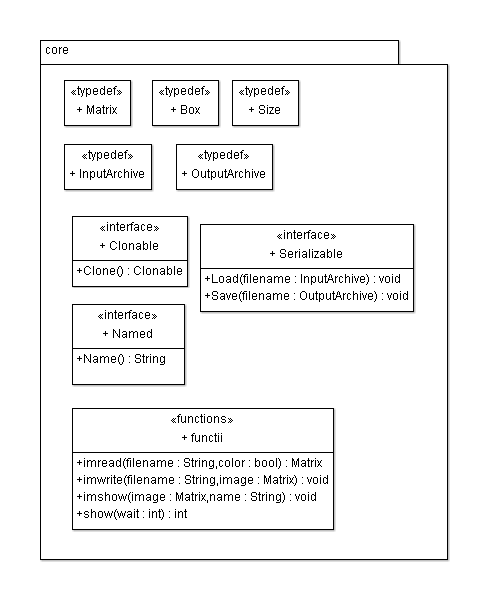
\includegraphics[width=0.95\textwidth]{uml/coreClassDiagram.png}
	\caption{core Class Diagram}
	\label{fig:coreClassDiagram}
\end{figure}

\subsection{Dataset}
Pachetul "dataset" conține clase care modelează baza de date pentru antrenament și implementează funcționalități de importare unor formate uzuale.
\begin{figure}[H]
	\centering
	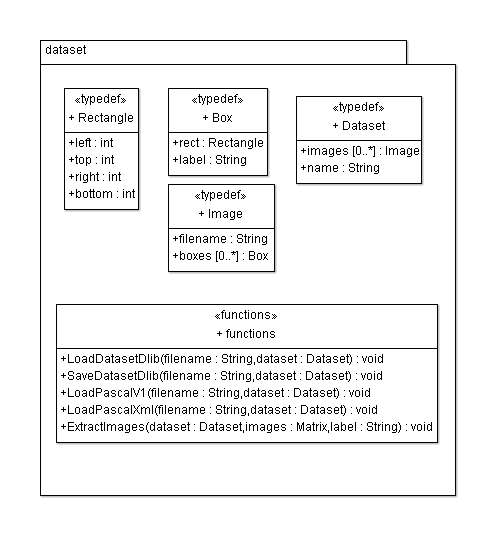
\includegraphics[width=1.0\textwidth]{uml/datasetClassDiagram.png}
	\caption{Diagrama de clase: dataset}
	\label{fig:datasetClassDiagram}
\end{figure}

\subsection{Image Pyramid}
Pachetul "image-pyramid" conține interfețe și implementări care servesc la construcția piramidei de imagini.
\begin{figure}[H]
	\centering
	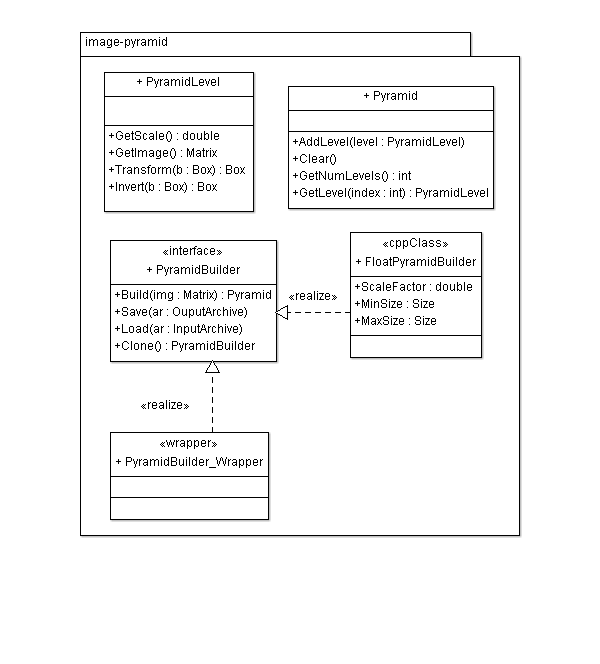
\includegraphics[width=1.00\textwidth]{uml/imagepyramidClassDiagram.png}
	\caption{Diagrama de clase: image-pyramid}
	\label{fig:imagepyramidClassDiagram}
\end{figure}


Clasa FloatPyramidBuilder construiește o piramida de imagini folosind ScaleFactor ca factor de scalare și MinSize, MaxSize ca criterii de terminare.

Metodele Transform si Invert din clasa PyramidLevel transforma coordonate din spațiul imaginii sursa în cel al nivelului, respectiv invers.

\subsection{Image Scanning}
Pachetul "image-scanning" conține interfețe și implementări care servesc la scanarea imaginilor
\begin{figure}[H]
	\centering
		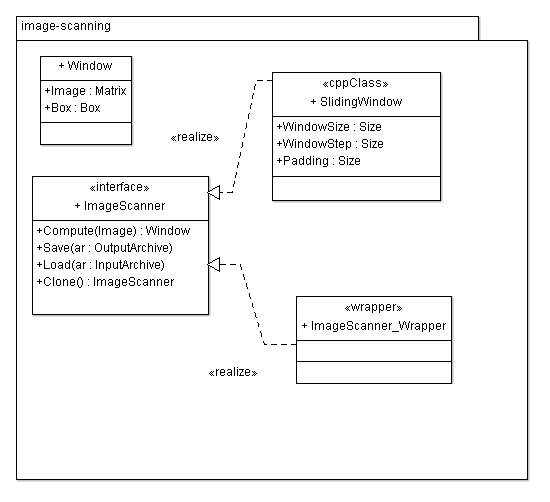
\includegraphics[width=1.00\textwidth]{uml/imagescanningClassDiagram.png}
	\caption{Diagrama de clase: image-scanning}
	\label{fig:imagescanningClassDiagram}
\end{figure}

\pagebreak
\subsection{Feature Extraction}
Pachetul "feature-extraction" conține interfețe și implementări care servesc la extragerea de trăsături din imagini.
\begin{figure}[H]
	\centering
		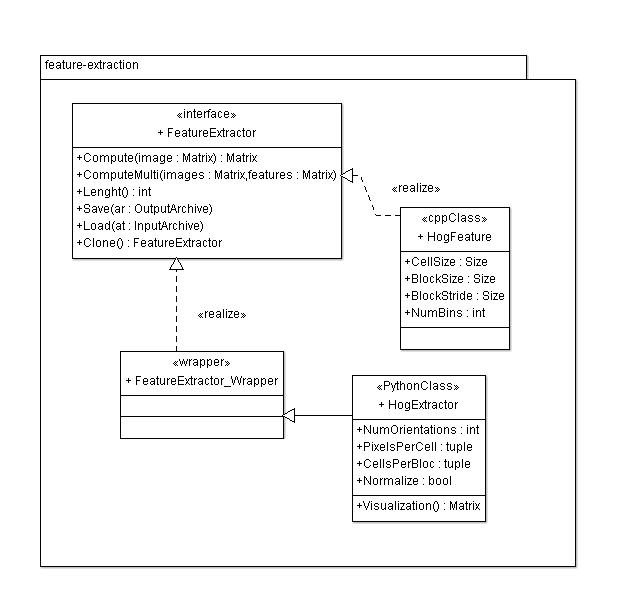
\includegraphics[width=1.00\textwidth]{uml/featureextractionClassDiagram.png}
	\caption{Diagrama de clase: feature-extraction}
	\label{fig:featureextractionClassDiagram}
\end{figure}

\pagebreak
\subsection{Classification}
Pachetul "classification" conține interfețe și implementări care servesc la clasificare și antrenarea clasificatorilor.
\begin{figure}[H]
	\centering
	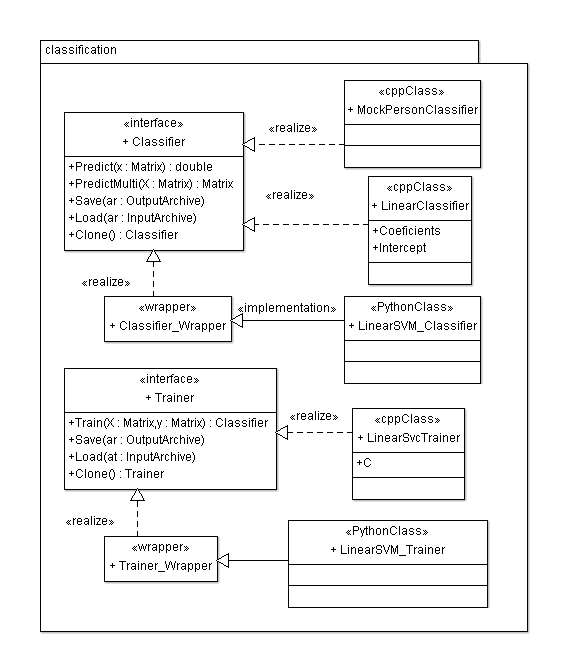
\includegraphics[width=1.00\textwidth]{uml/classificationClassDiagram.png}
	\caption{Diagrama de clase: classification}
	\label{fig:classificationClassDiagram}
\end{figure}

\subsection{Non Maxima Suppression}
Pachetul "non-maxima-suppression" conține interfețe și implementări care servesc la post-procesarea rezultatelor.
\begin{figure}[h]
	\centering
		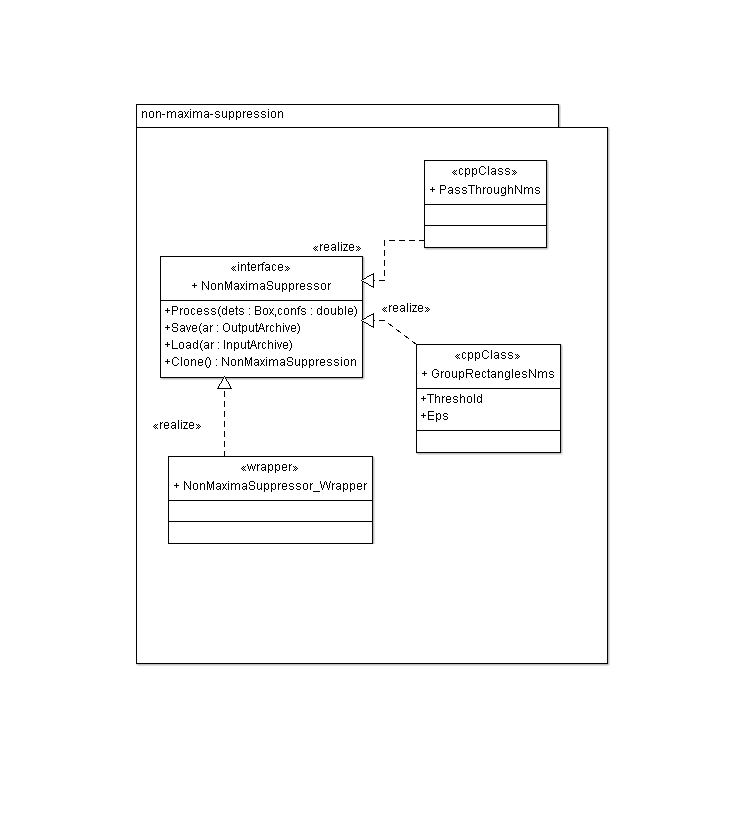
\includegraphics[width=1.00\textwidth]{uml/nonmaximasuppressionClassDiagram.png}
	\caption{Diagrama de clase: non-maxima-suppression}
	\label{fig:nonmaximasuppressionClassDiagram}
\end{figure}

\subsection{Detection}
Pachetul "detection" conține interfețe și implementări care servesc la recunoasterea obiectelor in imagini si la antrenarea algoritmilor.
\begin{figure}[H]
	\centering
		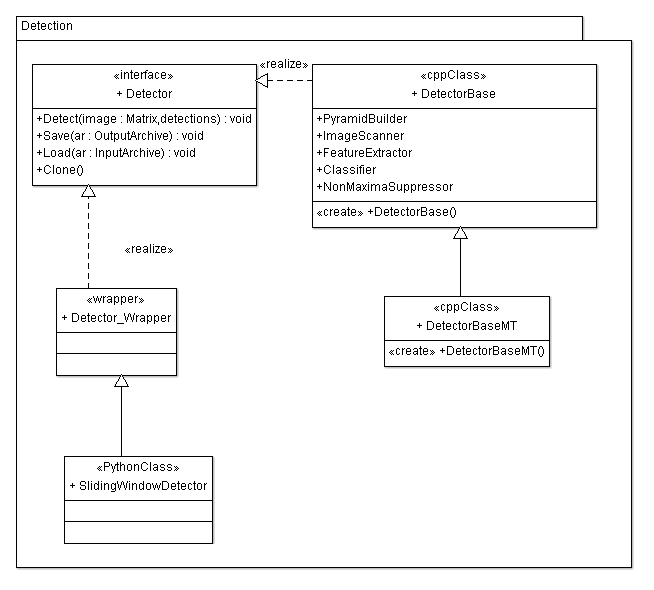
\includegraphics[width=1.00\textwidth]{uml/detectionClassDiagram.png}
	\caption{Diagrame de clase: detection}
	\label{fig:detectionClassDiagram}
\end{figure}
\begin{figure}[H]
	\centering
		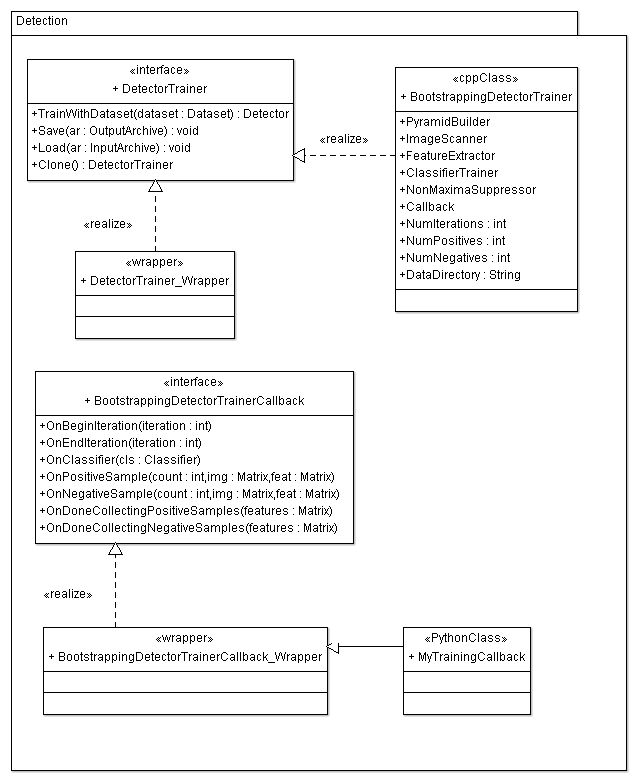
\includegraphics[width=1.00\textwidth]{uml/detection2ClassDiagram.png}
	\caption{Diagrama de clase: detection}
	\label{fig:detection2ClassDiagram}
\end{figure}

\pagebreak
\subsection{Python}
Pachetul "python" conține suportul necesar pentru interoperabilitatea cu limbajul Python.


\begin{figure}[H]
	\centering
		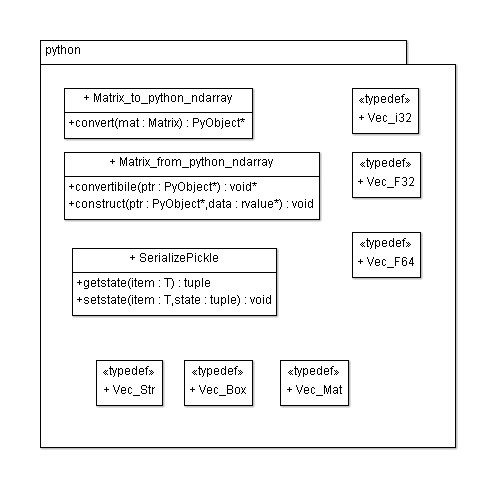
\includegraphics[width=1.00\textwidth]{uml/PythonClassDiagram.png}
	\caption{Diagrama de clase python}
	\label{fig:PythonClassDiagram}
\end{figure}




\pagebreak

\section{Interoperabilitatea cu Python}
\pagebreak

\section{Serializarea}
\pagebreak
%\chapter{}

%\chapter{Manual de utilizare}

%\chapter{Învățarea Automata}

Învățarea automata, o ramura a inteligentei artificiale, este preocupata de construirea și studierea unor sisteme care pot învață din date.

În 1959, Arthur Samuel a definit învățarea automata ca: "Domeniul de studiu care da calculatoarelor abilitatea de a învață fără să fie explicit programate"\cite{simon2013}.

Tom M. Mitchell o oferit o definiție mai formala: "Se spune despre un program ca a învățat din experienta ${E}$ cu privire la o clasa de acțiuni ${T}$ și o măsura de performanta ${P}$, în cazul în care performantele sale la sarcina ${T}$, măsurate prin ${P}$ se îmbunătățește cu experienta ${E}$."\cite{mitchell97}

Algoritmi de învățare automata se pot caracteriza în funcție de tipul de date cu care este antrenat și tipul de răspunsului dorit:
\begin{description}
	\item[Supervizată:]		
	Atunci când algoritmi sunt antrenați cu un set de date cu răspuns cunoscut și se dorește răspunsul în cazul unor date noi.
	
	\item[Nesupervizată:] 
	Atunci când algoritmi sunt antrenați cu un set de date cu răspuns necunoscut și se dorește găsirea unei structuri în setul de date.
\end{description}

În continuare vom discuta despre învățarea supervizată.

\subsection{Învățarea Supervizată}

Învățarea supervizata este sarcina învățării automate de a învață o funcție de evaluare din datele marcate de antrenament.
Datele de antrenament sunt constituite dintr-un set de exemple de antrenament, fiecare exemplu consta într-o pereche de valori de intrare și o valoare de ieșire dorita. Un astfel de algoritm analizează datele de antrenament și produce o funcție, care poate fii folosita pentru rezolvarea problemei în cazul unor date care nu au mai fost văzute.



Învățarea supervizata consta în învățarea unei funcții \( f:X \rightarrow Y \), unde \(X\) reprezinta domeniul datelor de intrare, iar \(Y\) domeniul datelor de ieșire, pentru un set de date de antrenare ${ \mathcal{D} = \{(x_i,y_i)|x_i \in X, y_i \in Y\}|_{i=1}^n }$ se doreste gasirea unei functiei ${ f(x_i) = y_i }$ și pentru \( x_i \notin \mathcal{D} \), adică date cu care nu a fost antrenat algoritmul.

 
În funcție de tipul de lui ${y}$, algoritmi de învățare supervizata pot fii clasificați astfel:
\begin{itemize}
	\item Regresie: atunci când răspunsul este o valoare numerica
	
	Exemplu: $${y \in \mathbb{R}}$$
	
	\item Clasificare: atunci când răspunsul este o valoare categorica.
	
	Exemplu: $${y \in \{0,1\}}$$ sau  $${y \in \{alb,negru,gri\}}$$
\end{itemize}

%\include{ProblemaRecunoasteriiFete}

%\include{ReteleNeuraleArtificiale}

%\include{ReteleNeuraleConvolutie}

%\include{Aplicatie}



%\include{Concluzii}
\chapter{Concluzii}

\nocite{*}
\bibliographystyle{plain}
\bibliography{Bibliografie}

\end{document}
